\documentclass[fleqn]{article}

%% Created with wxMaxima 23.05.1

\setlength{\parskip}{\medskipamount}
\setlength{\parindent}{0pt}
\usepackage{iftex}
\ifPDFTeX
  % PDFLaTeX or LaTeX 
  \usepackage[utf8]{inputenc}
  \usepackage[T1]{fontenc}
  \DeclareUnicodeCharacter{00B5}{\ensuremath{\mu}}
\else
  %  XeLaTeX or LuaLaTeX
  \usepackage{fontspec}
\fi
\usepackage{graphicx}
\usepackage{color}
\usepackage{amsmath}
\usepackage{grffile}
\usepackage{ifthen}
\newsavebox{\picturebox}
\newlength{\pictureboxwidth}
\newlength{\pictureboxheight}
\newcommand{\includeimage}[1]{
    \savebox{\picturebox}{\includegraphics{#1}}
    \settoheight{\pictureboxheight}{\usebox{\picturebox}}
    \settowidth{\pictureboxwidth}{\usebox{\picturebox}}
    \ifthenelse{\lengthtest{\pictureboxwidth > .95\linewidth}}
    {
        \includegraphics[width=.95\linewidth,height=.80\textheight,keepaspectratio]{#1}
    }
    {
        \ifthenelse{\lengthtest{\pictureboxheight>.80\textheight}}
        {
            \includegraphics[width=.95\linewidth,height=.80\textheight,keepaspectratio]{#1}
            
        }
        {
            \includegraphics{#1}
        }
    }
}
\newlength{\thislabelwidth}
\DeclareMathOperator{\abs}{abs}

\definecolor{labelcolor}{RGB}{100,0,0}

\begin{document}


\noindent
%%%%%%%%
%% INPUT:
\begin{minipage}[t]{4.000000em}\color{red}\bfseries
 --\ensuremath{\ensuremath{>}}	
\end{minipage}
\begin{minipage}[t]{\textwidth}\color{blue}
matrix:\ matrix(\\
\ [-2\ -\ lambda,a],\ \\
\ [9,-4*a\ -\ lambda]\\
);\\

\end{minipage}
%%%% OUTPUT:
\[\displaystyle \tag{matrix} 
\begin{pmatrix}\operatorname{-}lambda\operatorname{-}2 & a\\
9 & \operatorname{-}lambda\operatorname{-}4 a\end{pmatrix}\mbox{}
\]
%%%%%%%%%%%%%%%%
Найдем собственные числа матрицы, определяющей систему


\noindent
%%%%%%%%
%% INPUT:
\begin{minipage}[t]{4.000000em}\color{red}\bfseries
 --\ensuremath{\ensuremath{>}}	
\end{minipage}
\begin{minipage}[t]{\textwidth}\color{blue}
d:\ determinant(matrix);
\end{minipage}
%%%% OUTPUT:
\[\displaystyle \tag{d} 
\left( \operatorname{-}lambda\operatorname{-}2\right) \, \left( \operatorname{-}lambda\operatorname{-}4 a\right) \operatorname{-}9 a\mbox{}
\]
%%%%%%%%%%%%%%%%


\noindent
%%%%%%%%
%% INPUT:
\begin{minipage}[t]{4.000000em}\color{red}\bfseries
 --\ensuremath{\ensuremath{>}}	
\end{minipage}
\begin{minipage}[t]{\textwidth}\color{blue}
solve([d\ =\ 0],\ [lambda]);
\end{minipage}
%%%% OUTPUT:
\[\displaystyle \tag{\% o39} 
\operatorname{[}lambda\operatorname{=}\operatorname{-}\sqrt{4 {{a}^{2}}\operatorname{+}5 a\operatorname{+}1}\operatorname{-}2 a\operatorname{-}1\operatorname{,}lambda\operatorname{=
}\sqrt{4 {{a}^{2}}\operatorname{+}5 a\operatorname{+}1}\operatorname{-}2 a\operatorname{-}1\operatorname{]}\mbox{}
\]
%%%%%%%%%%%%%%%%
Вычислим произведение собственных значений матрицы


\noindent
%%%%%%%%
%% INPUT:
\begin{minipage}[t]{4.000000em}\color{red}\bfseries
 --\ensuremath{\ensuremath{>}}	
\end{minipage}
\begin{minipage}[t]{\textwidth}\color{blue}
prod:\ expand((-sqrt(4·a\^\ 2+5·a+1)-2*a-1)*(sqrt(4·a\^\ 2+5·a+1)-2·a-1));
\end{minipage}
%%%% OUTPUT:
\[\displaystyle \tag{prod} 
\operatorname{-}a\mbox{}
\]
%%%%%%%%%%%%%%%%
...


\noindent
%%%%%%%%
%% INPUT:
\begin{minipage}[t]{4.000000em}\color{red}\bfseries
 --\ensuremath{\ensuremath{>}}	
\end{minipage}
\begin{minipage}[t]{\textwidth}\color{blue}
expand(d);
\end{minipage}
%%%% OUTPUT:
\[\displaystyle \tag{\% o41} 
{{lambda}^{2}}\operatorname{+}4 a lambda\operatorname{+}2 lambda\operatorname{-}a\mbox{}
\]
%%%%%%%%%%%%%%%%


\noindent
%%%%%%%%
%% INPUT:
\begin{minipage}[t]{4.000000em}\color{red}\bfseries
 --\ensuremath{\ensuremath{>}}	
\end{minipage}
\begin{minipage}[t]{\textwidth}\color{blue}
dis:\ (4*a+2)\^\ 2\ -\ 4*a;
\end{minipage}
%%%% OUTPUT:
\[\displaystyle \tag{dis} 
{{\left( 4 a\operatorname{+}2\right) }^{2}}\operatorname{-}4 a\mbox{}
\]
%%%%%%%%%%%%%%%%


\noindent
%%%%%%%%
%% INPUT:
\begin{minipage}[t]{4.000000em}\color{red}\bfseries
 --\ensuremath{\ensuremath{>}}	
\end{minipage}
\begin{minipage}[t]{\textwidth}\color{blue}
radcan(dis);
\end{minipage}
%%%% OUTPUT:
\[\displaystyle \tag{\% o43} 
16 {{a}^{2}}\operatorname{+}12 a\operatorname{+}4\mbox{}
\]
%%%%%%%%%%%%%%%%


\noindent
%%%%%%%%
%% INPUT:
\begin{minipage}[t]{4.000000em}\color{red}\bfseries
 --\ensuremath{\ensuremath{>}}	
\end{minipage}
\begin{minipage}[t]{\textwidth}\color{blue}
wxplot2d([dis],\ [a,-2,1],\ [y,\ -5,\ 5]);
\end{minipage}
%%%% OUTPUT:
\[\displaystyle plot2d: some values will be clipped.
\mbox{}\]

\[\tag{\% t48} 
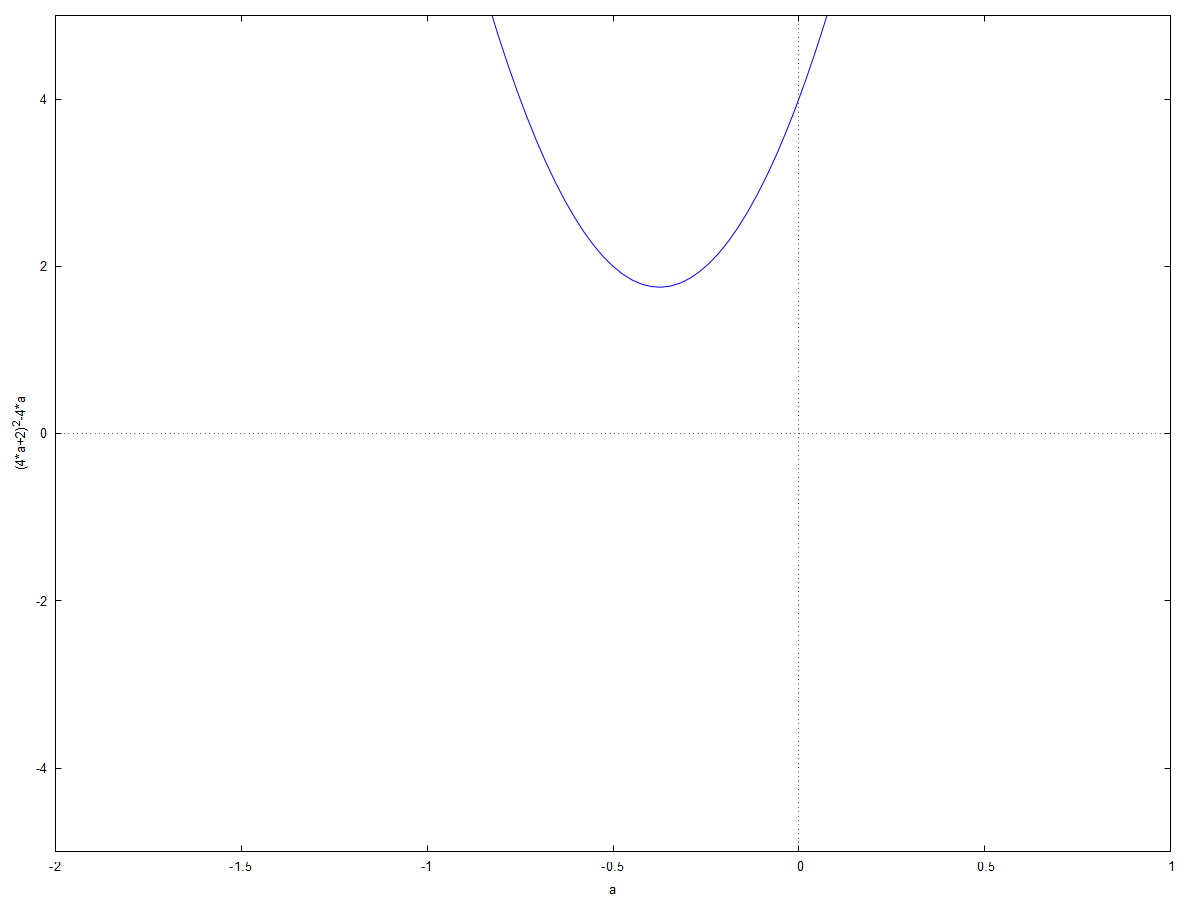
\includegraphics[width=.95\linewidth,height=.80\textheight,keepaspectratio]{difur1_img/difur1_1}\mbox{}\]

\[\tag{\% o48} 
\mbox{}
\]
%%%%%%%%%%%%%%%%
D\ensuremath{\sim }\ensuremath{>} 0 при всех а, поэтому оба корня вещественные.
Вырожденная матрица


\noindent
%%%%%%%%
%% INPUT:
\begin{minipage}[t]{4.000000em}\color{red}\bfseries
 --\ensuremath{\ensuremath{>}}	
\end{minipage}
\begin{minipage}[t]{\textwidth}\color{blue}
matrix([-2-lambda,0],\ [9,\ -lambda]);
\end{minipage}
%%%% OUTPUT:
\[\displaystyle \tag{\% o56} 
\begin{pmatrix}\operatorname{-}lambda\operatorname{-}2 & 0\\
9 & \operatorname{-}lambda\end{pmatrix}\mbox{}
\]
%%%%%%%%%%%%%%%%


\noindent
%%%%%%%%
%% INPUT:
\begin{minipage}[t]{4.000000em}\color{red}\bfseries
 --\ensuremath{\ensuremath{>}}	
\end{minipage}
\begin{minipage}[t]{\textwidth}\color{blue}
determinant(\%);\\

\end{minipage}
%%%% OUTPUT:
\[\displaystyle \tag{\% o57} 
\operatorname{-}\left( \left( \operatorname{-}lambda\operatorname{-}2\right)  lambda\right) \mbox{}
\]
%%%%%%%%%%%%%%%%


\noindent
%%%%%%%%
%% INPUT:
\begin{minipage}[t]{4.000000em}\color{red}\bfseries
 --\ensuremath{\ensuremath{>}}	
\end{minipage}
\begin{minipage}[t]{\textwidth}\color{blue}
solve([\%\ =\ 0],\ [lambda]);
\end{minipage}
%%%% OUTPUT:
\[\displaystyle \tag{\% o58} 
\left[ lambda\operatorname{=}\operatorname{-}2\operatorname{,}lambda\operatorname{=}0\right] \mbox{}
\]
%%%%%%%%%%%%%%%%


\noindent
%%%%%%%%
%% INPUT:
\begin{minipage}[t]{4.000000em}\color{red}\bfseries
 --\ensuremath{\ensuremath{>}}	
\end{minipage}
\begin{minipage}[t]{\textwidth}\color{blue}
load("plotdf");\\

\end{minipage}
%%%% OUTPUT:
\[\displaystyle \tag{\% o49} 
\mbox{}
\]\mbox{}\\"C:/maxima-5.47.0/share/maxima/5.47.0/share/dynamics/plotdf.lisp"



\noindent
%%%%%%%%
%% INPUT:
\begin{minipage}[t]{4.000000em}\color{red}\bfseries
 --\ensuremath{\ensuremath{>}}	
\end{minipage}
\begin{minipage}[t]{\textwidth}\color{blue}
plotdf([-2*x\ +a*y,\ 9*x-4*a*y],\ [x,\ y],\\
[parameters,\ "a\ =\ 0"],\ [trajectory\_at,\ 2,\ 1],\\
[tstep,\ 0.01],\ [x,\ -10,\ 10],\ [y,\ -10,\ 10],\\
[direction,\ forward],\ [nsteps,\ 300],\\
[sliders,\ "a=-10:10"],\ [versus\_t,\ 1])\$
\end{minipage}

\noindent%



\noindent
%%%%%%%%
%% INPUT:
\begin{minipage}[t]{4.000000em}\color{red}\bfseries
(\% i3)	
\end{minipage}
\begin{minipage}[t]{\textwidth}\color{blue}
wxplot2d([(-sqrt(4·a\^\ 2+5·a+1)-2*a-1)],\ [a,\ 0,\ 2],\ [y,\ -5,\ 2]);
\end{minipage}
%%%% OUTPUT:
\[\displaystyle plot2d: some values will be clipped.
\mbox{}\]

\[\tag{\% t3} 
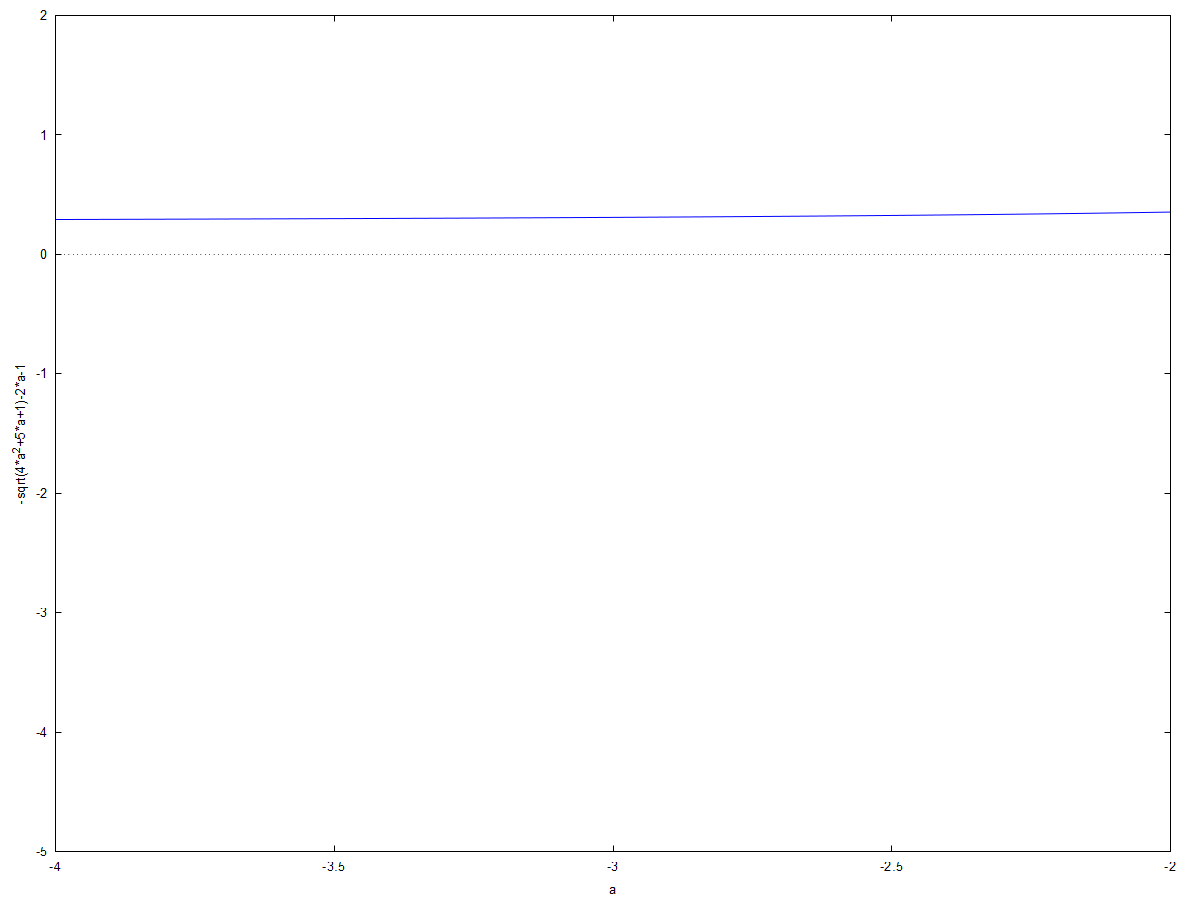
\includegraphics[width=.95\linewidth,height=.80\textheight,keepaspectratio]{difur1_img/difur1_2}\mbox{}\]

\[\tag{\% o3} 
\mbox{}
\]
%%%%%%%%%%%%%%%%
\end{document}
